\documentclass[]{tufte-handout}

% ams
\usepackage{amssymb,amsmath}

\usepackage{ifxetex,ifluatex}
\usepackage{fixltx2e} % provides \textsubscript
\ifnum 0\ifxetex 1\fi\ifluatex 1\fi=0 % if pdftex
  \usepackage[T1]{fontenc}
  \usepackage[utf8]{inputenc}
\else % if luatex or xelatex
  \makeatletter
  \@ifpackageloaded{fontspec}{}{\usepackage{fontspec}}
  \makeatother
  \defaultfontfeatures{Ligatures=TeX,Scale=MatchLowercase}
  \makeatletter
  \@ifpackageloaded{soul}{
     \renewcommand\allcapsspacing[1]{{\addfontfeature{LetterSpace=15}#1}}
     \renewcommand\smallcapsspacing[1]{{\addfontfeature{LetterSpace=10}#1}}
   }{}
  \makeatother

\fi

% graphix
\usepackage{graphicx}
\setkeys{Gin}{width=\linewidth,totalheight=\textheight,keepaspectratio}

% booktabs
\usepackage{booktabs}

% url
\usepackage{url}

% hyperref
\usepackage{hyperref}

% units.
\usepackage{units}


\setcounter{secnumdepth}{-1}

% citations
\usepackage{natbib}
\bibliographystyle{plainnat}


% pandoc syntax highlighting

% table with pandoc

% multiplecol
\usepackage{multicol}

% strikeout
\usepackage[normalem]{ulem}

% morefloats
\usepackage{morefloats}


% tightlist macro required by pandoc >= 1.14
\providecommand{\tightlist}{%
  \setlength{\itemsep}{0pt}\setlength{\parskip}{0pt}}

% title / author / date
\title[Ciencia abierta y reputación cientifica]{Handout Sobre Ciencia
Reproducible}
\author{Por Ricardo Palmma basado en textos de Sannchez Rodriguez}
\date{2022-12-22}


\begin{document}

\maketitle




\hypertarget{cruxe9ditos}{%
\section{Créditos}\label{cruxe9ditos}}

\(I^3\) INSTITUTO DE INGENIERÍA INDUSTRIAL UNIVERSIDAD NACIONAL DE CUYO

\footnote{
\includegraphics{images/iii.png}}

Artículo publicado en Open Access bajo los términos de Creative Commons
attribution Non Comercial License 3.0.

REVISIONES

\textbf{Título Original}: Ciencia reproducible: qué, por qué, cómo

Publicado en: REVISTA CIENTÍFICA DE ECOLOGÍA Y MEDIO AMBIENTE

ISSN 1697-2473 / Open access disponible en www.revistaecosistemas.net

\textbf{Autores:} F. Rodríguez-Sánchez1,*, A.J. Pérez-Luque2,\textbf{,
I. Bartomeus1,}, S. Varela3,**

\textbf{Traducción al Español: } Ricardo R. Palma4

\begin{enumerate}
\def\labelenumi{(\arabic{enumi})}
\tightlist
\item
  Departamento de Ecología Integrativa, Estación Biológica de Doñana
  (EBD-CSIC), Consejo Superior de Investigaciones Científicas, Avda.
  Américo Vespucio s/n, E-41092 Sevilla, España.
\item
  Laboratorio de Ecología (iEcolab), Instituto Interuniversitario
  Sistema Tierra (CEAMA), Universidad de Granada, Avda. del Mediterráneo
  s/n, Granada 18006, España.
\item
  Departamento de Ciencias de la Vida, Facultad de Biología, Ciencias
  Ambientales y Química, Universidad de Alcalá, Campus Universitario.
  Ctra. Madrid-Barcelona, Km. 33,600, 28805 Alcalá de Henares, Madrid,
  España.
\item
  Departamento de traducciones técnicas Centro de Estudios y
  Aplicaciones Logísticas \emph{CEAL} Facutlad de Ingeniería -
  Universidad Nacional de Cuyo Mendoza - Argentina
\end{enumerate}

\begin{itemize}
\tightlist
\item
  Autor de correspondencia: F. Rodríguez-Sánchez
  {[}\href{mailto:frodriguez.work@gmail.com}{\nolinkurl{frodriguez.work@gmail.com}}{]}
  ** Estos autores contribuyeron de manera equivalente y el orden se
  determinó ejecutando en R: sample(c(``AJPL'', ``IB'', ``SV'')).
  \textgreater{} Recibido el 08 de marzo de 2016 - Aceptado el 12 de
  junio de 2016
\end{itemize}

\hypertarget{objetivos}{%
\subsection{Objetivos}\label{objetivos}}

\hypertarget{resumen}{%
\subsection{Resumen}\label{resumen}}

La inmensa mayoría de los estudios científicos no son reproducibles:
resulta muy difícil, si no imposible, trazar todo el proceso de análisis
y obtención de resultados a partir de un conjunto de datos -- incluso
tratándose de los mismos investigadores. La trazabilidad y
reproducibilidad de los resultados son sin embargo condiciones
inherentes a la ciencia de calidad, y un requisito cada vez más
frecuente por parte de revistas y organismos financiadores de la
investigación. Los estudios científicos reproducibles incluyen código
informático capaz de recrear todos los resultados a partir de los datos
originales. De esta manera el proceso de análisis queda perfectamente
registrado, se reduce drásticamente el riesgo de errores, y se facilita
la reutilización de código para otros análisis. Pero la ciencia
reproducible no sólo acelera el progreso científico sino que también
reporta múltiples beneficios para el investigador como el ahorro de
tiempo y esfuerzo, o el incremento de la calidad e impacto de sus
publicaciones. En este artículo explicamos en qué consiste la
reproducibilidad, por qué es necesaria en ciencia, y cómo podemos hacer
ciencia reproducible. Presentamos una serie de recomendaciones y
herramientas para el manejo y análisis de datos, control de versiones de
archivos, organización de ficheros y manejo de programas informáticos
que nos permiten desarrollar flujos de trabajo reproducibles en el
contexto actual de la ecología.

\hypertarget{palabras-clave}{%
\subsubsection{Palabras clave}\label{palabras-clave}}

análisis de datos; ciencia abierta; ecoinformática; ecología;
programación; R; reproducibilidad

\footnote{\textbf{Abstract:} Most scientific papers are not
  reproducible: it is really hard, if not impossible, to understand how
  results are derived from data, and being able to regenerate them in
  the future (even by the same researchers). However, traceability and
  reproducibility of results are indispensable elements of highquality
  science, and an increasing requirement of many journals and funding
  sources. Reproducible studies include code able to regenerate results
  from the original data. This practice not only provides a perfect
  record of the whole analysis but also reduces the probability of
  errors and facilitates code reuse, thus accelerating scientific
  progress. But doing reproducible science also brings many benefits to
  the individual researcher, including saving time and effort, improved
  collaborations, and higher quality and impact of final publications.
  In this article we introduce reproducible science, why it is
  important, and how we can improve the reproducibility of our work. We
  introduce principles and tools for data management, analysis, version
  control, and software management that help us achieve reproducible
  workflows in the context of ecology.}

\hypertarget{key-words}{%
\subsubsection{Key words}\label{key-words}}

data analysis; ecoinformatics; ecology; open science; programming; R;
reproducibility

\hypertarget{introducciuxf3n}{%
\section{Introducción}\label{introducciuxf3n}}

¿Cuántas veces hemos querido revisitar un análisis estadístico meses o
años después y no hemos sido capaces, bien porque no recordamos cómo
hacerlo o los datos no están fácilmente disponibles? ¿Cuánto tiempo
perdemos en rehacer análisis estadísticos, figuras o tablas tras
corregir un error en los datos, o siguiendo las recomendaciones de un
revisor? ¿Cuánto tiempo invertimos intentando implementar un nuevo
método de análisis a partir de la escueta descripción proporcionada en
un artículo? ¿Cuántas veces hemos intentado recabar datos
infructuosamente porque los autores han perdido los datos, su formato es
ilegible hoy en día, o simplemente se niegan a compartirlos?

\begin{marginfigure}
\textbf{Pensa en esto \ldots{}}

Sabemos que el teorema fundamental del cálculo infinitesimal se expresa
así.

for \(x\) in \([a, b]\):
\[\frac{d}{dx}\left( \int_{a}^{x} f(u)\,du\right)=f(x).\]

Pero estaríamos condenado de deducirlo nuevamente si alguien no lo
hubiese escrito gentilmente para nosostros hace varios siglos atrás,
sólo para que pudiesemos mirar más adelante sobre hombros de gigantes..
\end{marginfigure}

Todas estas escenas son desgraciadamente frecuentes en el día a día de
los científicos, y evidencian un grave problema de reproducibilidad en
ciencia (Peng 2011). La inmensa mayoría de los artículos científicos no
son reproducibles, esto es, resulta muy difícil o imposible trazar
claramente el proceso de obtención de los resultados y volver a
obtenerlos (reproducirlos) ¡incluso tratándose del mismo equipo de
autores! En este artículo discutimos por qué los resultados científicos
deben ser reproducibles, presentamos las ventajas de adoptar flujos de
trabajo reproducibles, e introducimos las principales herramientas para
ello.

\hypertarget{quuxe9-es-la-ciencia-reproducible}{%
\section{¿Qué es la ciencia
reproducible?}\label{quuxe9-es-la-ciencia-reproducible}}

\emph{``A scientific article is advertising, not scholarship. The actual
scholarship is the full software environment, code and data, that
produced the result.''} \textbf{\emph{Claerbout y Karrenbach (1992).}}

La ciencia se caracteriza por seguir unas pautas metodológicas que
garantizan su validez epistemológica (Pigliucci y Boudry 2013). La
confrontación rigurosa de hipótesis con evidencias empíricas
(observacionales o experimentales) y el escrutinio público de los
resultados contribuyen a garantizar que las conclusiones sean ciertas.
Es por ello que los artículos científicos tienen una sección de métodos
explicando los pasos seguidos en la recolección y análisis de datos.
Esta información resulta crucial para examinar la veracidad y robustez
de las conclusiones del artículo, así como para permitir futuras
repeticiones del estudio por otros autores. Sin embargo, en la mayoría
de ocasiones la escueta descripción verbal que aparece en la sección de
métodos resulta insuficiente para conocer todos los detalles del
análisis (Ince et al.~2012, Fig. 1). Este problema resulta cada vez más
acuciante con el aumento de la complejidad de los análisis estadísticos
(Michener y Jones 2012).

Un estudio científico es reproducible si el texto del artículo viene
acompañado de código (texto interpretable por un ordenador) que permite
recrear exactamente a partir de los datos originales todos los
resultados y figuras incluidos en el artículo (Peng 2011; Marwick 2016).
El concepto es por tanto diferente al de repetibilidad, que se refiere a
la posibilidad de replicar el mismo estudio (con nuevos datos) a partir
de la información proporcionada en el artículo. La reproducibilidad se
relaciona principalmente con la transparencia, trazabilidad, y
completitud del protocolo seguido para llegar a unos resultados
concretos a partir de un conjunto de datos determinado. La
reproducibilidad no es una cualidad binaria sino un gradiente que va
desde trabajos totalmente irreproducibles (que sólo contienen el texto,
tablas y figuras finales) a estudios perfectamente reproducibles donde
la integración de texto, código y datos permite regenerar fácilmente el
resultado final a partir de los datos originales (e.g.~Goring et
al.~2013; FitzJohn et al.~2014, Fig. 1).

\#¿Por qué es necesaria la reproducibilidad en ciencia?

``Every analysis you do on a dataset will have to be redone 10-15 times
before publication. Plan accordingly.'' Trevor A. Branch.

La reproducibilidad es un pilar fundamental del método científico: los
resultados deben estar basados en datos y evidencias perfectamente
contrastables. De hecho, ningún estudio científico puede garantizar que
sus resultados sean correctos, pero sí reproducibles (Peng 2011). La
reproducibilidad es por tanto una garantía de transparencia y calidad:
los artículos reproducibles están mejor blindados frente a errores, y
cuando los contienen son detectados y corregidos más fácilmente (Check
Hayden 2015). Además, la reutilización de código pre-existente por parte
de otros autores contribuye a acelerar el progreso científico. En los
últimos años ha aumentado la presión por incrementar la reproducibilidad
de los trabajos científicos, tras la creciente detección de errores
graves en artículos que carecen de garantías de reproducibilidad
(Anónimo 2014a; b; Alberts et al.~2015). De hecho, el número de revistas
y fuentes de financiación que requieren la publicación de datos y código
no para de crecer (Stodden et al.~2013).

Pero la reproducibilidad no debería ser vista como una obligación
impuesta externamente, sino como una oportunidad de mejorar nuestra
manera de hacer ciencia y aumentar la contribución de nuestros trabajos
al avance científico general. Hacer ciencia reproducible trae consigo
múltiples ventajas para el investigador (ver Tabla 1), a pesar del
esfuerzo inicial que siempre conlleva aprender nuevas técnicas de
trabajo.

Para empezar, tener flujos de trabajo reproducibles evita muchos de los
problemas planteados al comienzo de este artículo. Por ejemplo, tras
corregir un error en los datos o introducir nuevas observaciones podemos
volver a generar -sin ningún esfuerzo extra- todas las tablas, figuras y
resultados de un trabajo. Esto no sólo ahorra tiempo sino que disminuye
drásticamente los errores en el manuscrito final. Igualmente, la
existencia de un código que documenta fielmente el proceso de análisis
facilita tanto la escritura del manuscrito como su interpretación por
coautores, revisores y lectores finales (Markowetz 2015). Además, dicha
transparencia le da un sello de calidad al trabajo y facilita su
aceptación, incrementando su impacto posterior en términos de citas y
reconocimiento (Piwowar et al.~2007; Vandewalle 2012). Por ejemplo, la
revista Molecular Ecology menciona en sus instrucciones a los autores
que ``los artículos con archivado de datos y código son más valiosos
para investigaciones futuras, por lo que, a igualdad de condiciones, se
les dará mayor prioridad para su publicación''. La existencia de un
código ordenado y bien estructurado permitirá además su reutilización en
proyectos posteriores, ahorrando tiempo y esfuerzos al equipo de
investigación (Garijo et al.~2013). Además, compartir públicamente el
código con el que generamos unos resultados puede ayudarnos a
identificar errores (idealmente antes de su publicación) y abrir nuevas
líneas de colaboración (Hampton et al.~2015).

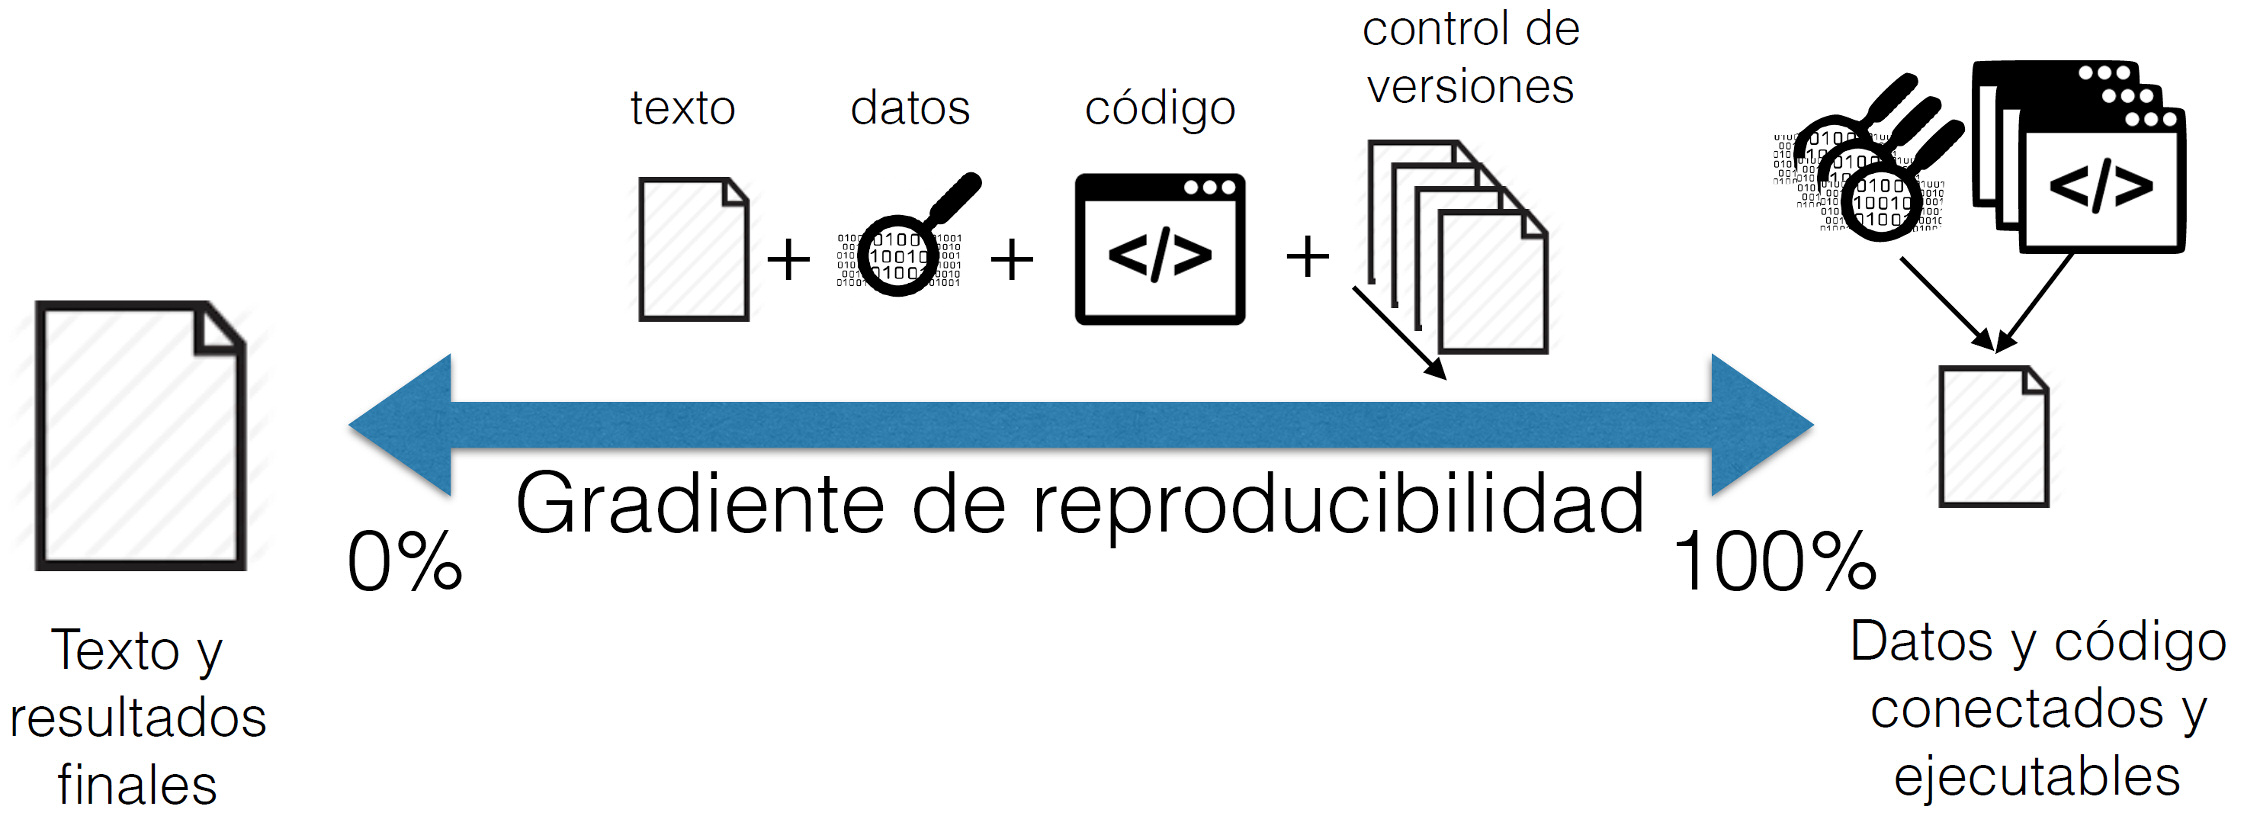
\includegraphics{images/fig_-000.jpg} \footnote{Figura 1. La
  reproducibilidad no es una cualidad binaria sino un gradiente (Peng
  2011). Los artículos científicos que sólo contienen el texto,
  resultados y figuras finales (por ejemplo en un único archivo pdf) son
  los menos reproducibles: es imposible reconstruir detalladamente el
  proceso de análisis desde los datos originales hasta los resultados
  finales. La publicación de los datos y/o el código empleado para el
  análisis contribuyen a mejorar la reproducibilidad. Igualmente, la
  existencia de un sistema de control de versiones (como git) permite
  reconstruir perfectamente la historia del proyecto. Finalmente, en el
  extremo del gradiente de reproducibilidad se encuentran los documentos
  dinámicos (por ejemplo, Rmarkdown o IPython) que integran
  perfectamente texto, datos y código ejecutable.}

Figure 1. Reproducibility is not a binary quality but a gradient (Peng
2011). Scientific articles that contain only the final text, results and
figures (e.g.~in a single pdf document) are the least reproducible - it
is impossible to reconstruct the whole analytic process from data to
results. Publication of the data and/or code used for the analysis
greatly improve reproducibility. Likewise, usage of a version control
system (like git) permits navigating through the complete history of the
project. Finally, the most reproducible studies are those using dynamic
reports (e.g.~Rmarkdown or IPython notebooks) that integrate text, code
and data in a fully executable environment.

Tabla 1. Ventajas para el investigador derivadas de la adopción de
flujos de trabajo reproducibles. Table 1. Personal benefits for
researchers from developing reproducible workflows.

Beneficios de la ciencia reproducible para el investigador

Beneficios para la organiacion patrocinante

• La utilización de código permite la automatización: ejecución de
tareas repetitivas sin esfuerzo

• El sistema de bibliotecas institucional simplifica la generación de
tesauros y la indexación correcta

• Reducción drástica del riesgo de errores

• Posibilidades de desarrollo para nuevos tesistas en base a errores
detectados

• Muy fácil corregir y regenerar resultados, tablas y figuras

• El investigador se centra en el textos que permite comunicar a la
comunidad epistémica y se olvida del formato (documento, pagina web,
diapositiva, poster). Se conservando la línea editorial de la
Universidad, logos, filiación, etc

• Los flujos de trabajo reproducibles facilitan la colaboración

• La mayor porductividad, visibilidad y calidad de los trabajos apoyan a
los procesos de acreditación de la institución.

• Mayor facilidad para escribir artículos al tener registro exhaustivo
de todo el proceso de análisis

• Aporta transparencia a los procesos de los modelos de triple hélice en
los que interviene la academia.

• La publicación del código y modelos utilizados ayuda a detectar
errores antes de la publicación definitiva • La publicación del código
facilita el proceso de revisión

• Preserva para generaciones futuras los entretelones del proceso de
avance cientifico de una comunidad epistémica.

\footnote{La reproducibilidad es un sello de calidad y aumenta la
  probabilidad de aceptación (cuando no es simplemente requerida) La
  reproducibilidad aumenta el impacto de las publicaciones (citas,
  reconocimiento, reutilización, coautorías) Ahorro de tiempo y esfuerzo
  al reutilizar modelos código y conjeturas en otros proyectos}

\hypertarget{cuxf3mo-hacer-ciencia-reproducible}{%
\section{Cómo hacer ciencia
reproducible}\label{cuxf3mo-hacer-ciencia-reproducible}}

\emph{``You can't reproduce if you don't understand where a number came
from. You can't reproduce what you don't remember. And trust me: you
won't. You can't reproduce what you've lost. What if you need access to
a file as it existed 1, 10, 100, or 1000 days ago?''}
\textbf{\emph{Bond-Lamberty (2014).}}

Adoptar un flujo de trabajo reproducible (Fig. 2) requiere un esfuerzo
inicial importante. Es necesario familiarizarse con diversas
herramientas (bases de datos, programación, sistemas de control de
versiones) lo cual lleva su tiempo. Recibir una formación adecuada y
temprana (idealmente previa a la realización del proyecto de máster o
doctorado) facilita mucho las cosas. Dado que el interés por la ciencia
reproducible es bastante reciente, en nuestro país la formación es aún
escasa, aún más en el campo de la ecología. Pero existen cursos, libros
y material de aprendizaje fácilmente disponibles (ver Apéndice 1).

La reproducibilidad no es una cualidad binaria sino un gradiente (Fig.
1) y conviene implementarla paso a paso en nuestra investigación para
facilitar la transición (Tabla 2). Un ejemplo extremo de
irreproducibilidad sería aquel donde los datos son manipulados en una
hoja de cálculo (e.g.~Microsoft Excel, LibreOffice Calc), posteriormente
analizados manualmente en programas estadísticos (como Statistica o
SPSS), el manuscrito redactado en un procesador de texto (e.g.~Microsoft
Word, Google Docs), las figuras realizadas en un programa gráfico
(e.g.~SigmaPlot, Adobe Illustrator, Photoshop), y los valores de las
tablas copiados a mano. Afortunadamente, cada vez es más frecuente que
los análisis se hagan mediante código (mayoritariamente R o Python), lo
cual representa un avance importante en cuanto a reproducibilidad. Sin
embargo, dicho flujo de trabajo incluye todavía múltiples pasos manuales
que rompen su dinamismo, no dejan registro de las operaciones
realizadas, y abren la puerta a la introducción de errores (por ejemplo,
al copiar manualmente múltiples valores a una tabla). En el otro extremo
de este gradiente de reproducibilidad estarían los análisis puramente
integrados donde el trabajo final puede ser reconstituido a partir de
los datos originales con un solo comando o clic del ratón (Fig. 1). A
continuación presentamos los elementos más importantes de un flujo de
trabajo reproducible (Fig. 2, Tabla 2) e introducimos las principales
herramientas disponibles para el manejo de datos, análisis de datos
mediante código, control de versiones, la organización de los archivos,
y el manejo de las dependencias de software externo. En el Apéndice 1
hemos incluido un listado de recursos que profundizan más en cualquiera
de estos aspectos.

\hypertarget{recolecciuxf3n-y-manejo-de-datos}{%
\subsection{Recolección y manejo de
datos}\label{recolecciuxf3n-y-manejo-de-datos}}

El proceso de recolección y manejo de datos resulta crucial, ya que
cualquier error en esta primera etapa se propagará hasta los resultados
finales. Por tanto es muy importante garantizar la calidad de este
proceso, que podría dividirse en cinco etapas (Michener y Jones 2012):

\hypertarget{planificaciuxf3n}{%
\subsubsection{Planificación}\label{planificaciuxf3n}}

Una buena planificación es la mejor forma de asegurar la calidad de los
datos, multiplicando su valor durante y después de finalizado el
proyecto (Rüegg et al.~2014). Muchas instituciones (como la National
Science Foundation de Estados Unidos) requieren la presentación de un
`data management plan' con cada proyecto
(\url{http://www.nsf.gov/bio/biodmp.jsp}). Dicho plan debe incluir
información detallada acerca de qué datos se van a obtener y cómo van a
recogerse, almacenarse y compartirse (Michener y Jones 2012; Michener
2015) (por ejemplo véase \url{https://www.dataone.org/}
sites/all/documents/DMP\_Copepod\_Formatted.pdf). Para ello, existen
herramientas como DMPTool (\url{https://dmptool.org/}) muy útiles para
elaborar esta planificación.

\hypertarget{recolecciuxf3n}{%
\subsubsection{Recolección}\label{recolecciuxf3n}}

El proceso de obtención de datos ecológicos varía enormemente según el
tipo de estudio, desde la captura de organismos en el campo hasta la
descarga de imágenes de satélite. A pesar de esta heterogeneidad, un
principio común a seguir es intentar conservar los datos brutos en su
estado original de la mejor manera posible (por ejemplo, insectos
capturados en un museo o una colección, fichas de campo en un archivo
seguro, imágenes o capas GIS en un repositorio), con un identificador
único. Esto nos permite establecer claramente qué conjunto de datos se
ha utilizado para un análisis, así como revisar/reutilizar estos datos
en el futuro. Igualmente, la metodología de obtención de datos debe
quedar perfectamente registrada.

\hypertarget{descripciuxf3n-del-conjunto-de-datos-metadatos}{%
\subsubsection{Descripción del conjunto de datos
(metadatos)}\label{descripciuxf3n-del-conjunto-de-datos-metadatos}}

Todo conjunto de datos debe ir acompañado de una descripción detallada
de lo que representa cada variable, cómo y dónde se tomó, en qué
unidades está medida, cuándo se tomaron los datos, quien los tomó, etc.
Esta información, conocida como metadatos, resulta necesaria para una
correcta interpretación de los datos (Michener et al.~1997), y además
multiplica su utilidad favoreciendo la reutilización (Fegraus et
al.~2005; Alonso y Valladares 2006; Rüegg et al.~2014).

\begin{figure*}
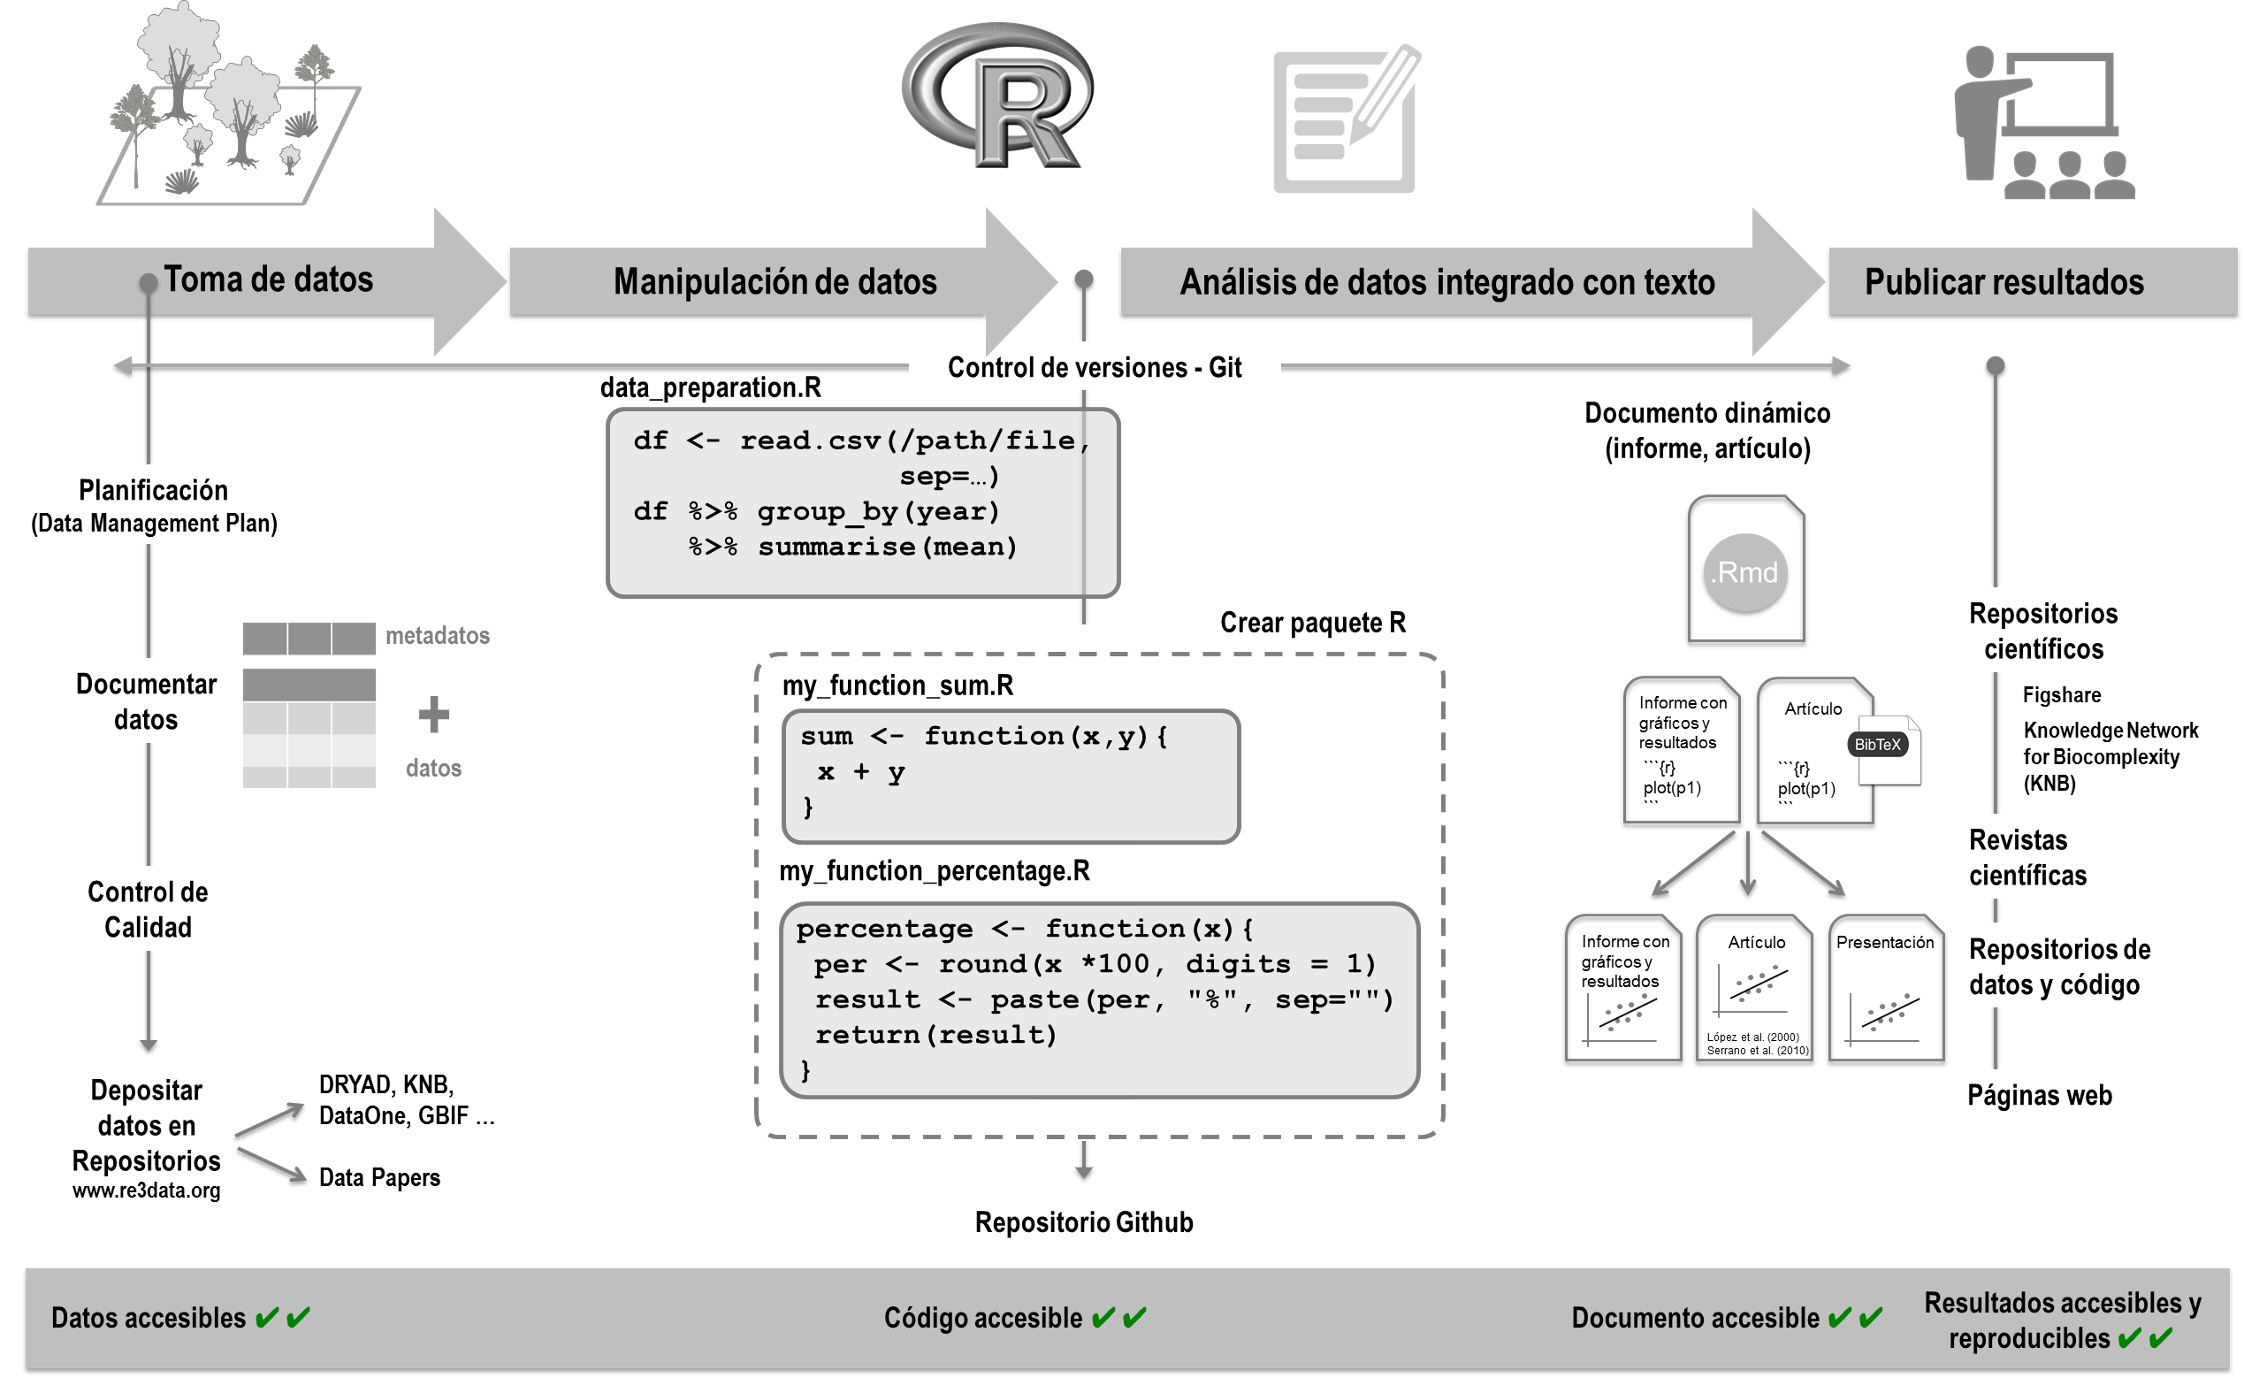
\includegraphics[width=1\linewidth]{images/fig_-001} \caption[Fig]{Fig. 2 - Flujo asistido de implementación.}\label{fig:unnamed-chunk-2}
\end{figure*}

Figura 2. Esquema de un flujo de trabajo reproducible. En primer lugar,
los datos se recogen según un protocolo bien diseñado, se documentan con
metadatos (e.g.~usando el estándar EML, `Ecological Metadata Language'),
se someten a un control de calidad (idealmente de manera automática,
esto es, mediante funciones de código), y se almacenan en un repositorio
de datos en la nube. Después procederíamos al análisis, siempre
utilizando `scripts' para manipular los datos, y creando funciones que
pueden almacenarse en un paquete (para facilitar su documentación y
posterior reutilización). El análisis propiamente dicho se haría
mediante documentos de Rmarkdown o IPython que integran texto, código y
resultados (tablas y figuras). Estos documentos pueden convertirse
fácilmente en presentaciones, páginas web, o artículos científicos
plenamente reproducibles. Figure 2. Sketch of a reproducible data
analysis workflow. First, data are collected following a well-designed
plan, documented with metadata (e.g.~using EML, the Ecological Metadata
Language), quality-controlled (ideally through automated functions), and
stored in an online repository. For the data analysis, we would always
use scripts for data wrangling and preparation, as well as functions to
perform repeated tasks. These functions could be wrapped into a package
to facilitate their share and reuse. The actual analysis would be done
using literate programming (e.g.~Rmarkdown or IPython). These documents
integrate text, code and results (tables and figures) and are fully
executable, so they can be easily converted into presentations, web
pages, or fully reproducible manuscripts.

Aunque los metadatos pueden alojarse en un simple fichero de texto, es
muy conveniente utilizar un sistema estándar pues facilita la
validación, integración y síntesis de los datos de manera automatizada
(Alonso y Valladares 2006).

\footnote{El hecho de escribir tus paper con procesadores de texto como
  \emph{MS Word} y guardarlos en formato PDF para publicarlos en
  journals o enviarlos a congresos genera una archivo que desde el punto
  de vista de los metadatos es \textbf{``mudo''}. Esto es aún más cierto
  si utilizas \emph{MS 365}. Crear datos con R-Cran o Jupyer Notebooks
  incrementa tu reputación (índice h) y garantiza prestigio para la
  organización en la que registres tu filiación.}

Existen diferentes estándares de metadatos en función del propósito y la
disciplina científica. En el terreno de las ciencias aplicadas todos los
Journals de Elsevier que utilizan la plantilla Lecture Notes in Computer
Sciences y las plantillas que ofrece la IEEE facilitan la busqueda y
clasificación del conocimiento. En ecología y ciencias de la vida en
general existe el estándar llamado `Ecological Metadata Language' (EML)
(\url{http://knb.ecoinformatics.org/software/eml/}) que se utiliza por
ejemplo en las redes de seguimiento ecológico a largo plazo (LTER,
Long-Term Ecological Research; Vanderbilt et al.~(2015)). Existen varias
herramientas para crear o editar metadatos, como Morpho
(\url{http://knb.ecoinformatics.org/morphoportal.jsp}), DEIMS
(\url{https://data.lter-europe.net/deims/}, utilizado en la red LTER), o
el paquete de R eml (\url{https://github.com/ropensci/EML/}).

\hypertarget{control-de-calidad}{%
\subsubsection{Control de calidad}\label{control-de-calidad}}

El control de calidad de los datos es un paso imprescindible pero
frecuentemente obviado. Siempre se introducen errores, ya sea en la toma
de datos en el campo o al introducirlos en un ordenador, y es importante
detectarlos y depurarlos. La utilización de plantillas que restrinjan el
tipo de datos introducido (e.g.~fecha en un formato determinado, valores
numéricos dentro de un rango determinado, especie a elegir de un listado
predefinido) evita la introducción de muchos errores desde el principio.
En cualquier caso, es conveniente realizar un control de calidad final
comprobando que todos los datos se ajustan a unos valores adecuados o
razonables. Este control de calidad puede hacerse de manera reproducible
e iterativa mediante funciones de importación de datos que incluyen
tests para comprobar la validez de los datos (e.g.~ver
\url{http://ropensci.org/blog/2015/06/03/baad}).

\footnote{Además, es importante seguir algunas normas básicas de
  estructuración de la base de datos (Wickham 2014) para facilitar su
  análisis posterior (e.g.~ver \url{http://kbroman.org/dataorg/} o
  \url{http://www.datacarpentry.org/spreadsheet-ecology-lesson/}).}

\hypertarget{preservaciuxf3n}{%
\subsubsection{Preservación}\label{preservaciuxf3n}}

Finalmente, debemos buscar la forma de asegurar que nuestros datos
seguirán estando disponibles a largo plazo. Un estudio reciente (Vines
et al.~2014) estimó que la disponibilidad de los datos se reduce con el
tiempo a una alarmante tasa anual del 17 \%. En muchos casos, la
dificultad de acceso a los datos se debe a su almacenamiento en formatos
propietarios o dispositivos digitales obsoletos; otras veces simplemente
se extravían. Actualmente, la mejor manera de asegurar la persistencia
de los datos a largo plazo (White et al.~2013; Hart et al.~2016) es
alojarlos en formato abierto (e.g.~txt o csv para datos tabulados, png
para imágenes) en un repositorio oficial de los muchos que hay
disponibles (ver \url{http://www.re3data.org/}). Muchos de estos
repositorios están orientados a la difusión pública de los datos, pero
otros permiten alojamiento privado (e.g.~Figshare, KNB, Open Science

Framework). Estos repositorios otorgan un identificador único y
persistente (DOI, Digital Object Identifier) a los datos, facilitando su
reutilización y citación. Existen múltiples programas que permiten
subir, actualizar y descargar datos fácilmente desde estos repositorios
(e.g.~ver \url{http://ropensci.org/packages/\#data_publication}). El
alojamiento en la nube representa por tanto la mejor opción para la
conservación de los datos (Hart et al.~2016).

Tabla 2. Criterios y recomendaciones para incrementar la
reproducibilidad de nuestra investigación. Table 2. Checklist of
criteria and recommendations to increase the reproducibility of our
research.

Criterios de reproducibilidad

Los datos originales están disponibles Los datos han sido revisados y
validados (preferiblemente de manera automática) Existe un conjunto de
metadatos explicando la estructura, formato y contenido de los datos Los
datos están almacenados en formato abierto (e.g.~txt, csv) Los datos se
han subido a un repositorio en la nube Todo el análisis y manejo de
datos se hace mediante código (`scripts') El código es inteligible y
está bien documentado El código genera las tablas y figuras finales
Todos los resultados del trabajo se actualizan dinámicamente (nunca
manualmente) Todos los archivos importantes (datos, código) están
versionados (por ejemplo usando git) Existe copia de seguridad de todos
los archivos importantes en (cuasi) tiempo real Todos los archivos
relacionados con el proyecto están dentro del mismo directorio Existen
subdirectorios independientes para los datos, código, figuras, etc. Los
datos brutos están separados de los datos derivados El código utiliza
funciones que se definen en un fichero independiente Se han escrito
tests que comprueban que las funciones actúan correctamente Existe un
`script' maestro que ejecuta todos los pasos del análisis ordenadamente
Existe un documento README que explica los objetivos y organización del
proyecto Existe un registro detallado de todas las dependencias de
software externo (incluyendo la versión) Es posible instalar todas esas
dependencias en el futuro o en otro ordenador Tanto el manuscrito como
los datos y código son públicos Se especifica el tipo de licencia que
tienen los datos y el código

\hypertarget{anuxe1lisis-de-datos-y-documentos-dinuxe1micos}{%
\subsection{Análisis de datos y documentos
dinámicos}\label{anuxe1lisis-de-datos-y-documentos-dinuxe1micos}}

Para que un estudio sea reproducible, todo el análisis debe realizarse
mediante `scripts' de código, desde la manipulación de datos hasta la
generación de tablas y figuras. Eso significa que debemos evitar hacer
ningún cambio directamente sobre los datos originales (e.g.~en una hoja
de cálculo como Microsoft Excel): los datos originales son intocables, y
cualquier modificación posterior debe realizarse mediante código de
manera que quede un registro de todos los cambios realizados.

La utilización de código trae consigo una serie de ventajas frente al
análisis manual mediante clics. En primer lugar, el análisis manual es
totalmente irreproducible, a diferencia del código que es interpretable
tanto para humanos como computadoras. El código contiene un registro
perfecto de todos los pasos seguidos en el análisis, muy útil para
compartir con colaboradores o reutilizar algún tiempo después (siempre
que podamos reproducir el entorno de computación, véase sección de
dependencias externas más abajo). Además, la utilización de código
permite automatizar tareas, ahorrando tiempo al investigador.

En muchas disciplinas científicas el lenguaje de programación dominante
desde hace años es R (www.r-project.org). R es un lenguaje gratuito, de
código abierto, inicialmente dirigido al análisis de datos y la
visualización, pero cuyos usos no paran de crecer gracias a una
comunidad muy activa de usuarios-desarrolladores que contribuyen sus
propios `paquetes' con funciones (ver
\url{https://cran.r-project.org/web/packages/available_packages_}
by\_name.html). Además de R, existen otros lenguajes de programación
bastante extendidos como Python, C, C++, MATLAB, etc. (Bass y Nixon
2008).

La aparición en el último lustro de herramientas para generar documentos
dinámicos a partir de un conjunto de datos y código (knitr y rmarkdown
en R, IPython para Python, Jupyter para múltiples lenguajes) ha supuesto
una auténtica revolución en el campo de la ciencia reproducible. Estos
programas integran texto y código de manera que es posible regenerar
todas las tablas, figuras y resultados presentes en un artículo, libro o
informe con un solo clic (Fig. 3). Ello nos libra por tanto de tener que
volver a copiar manualmente todos los valores de una tabla o rehacer
figuras con cada iteración del análisis. Por tanto, utilizar documentos
dinámicos no sólo ahorra tiempo sino que también reduce la probabilidad
de cometer errores: todos los resultados son perfectamente trazables a
partir de los datos originales.

\begin{figure*}
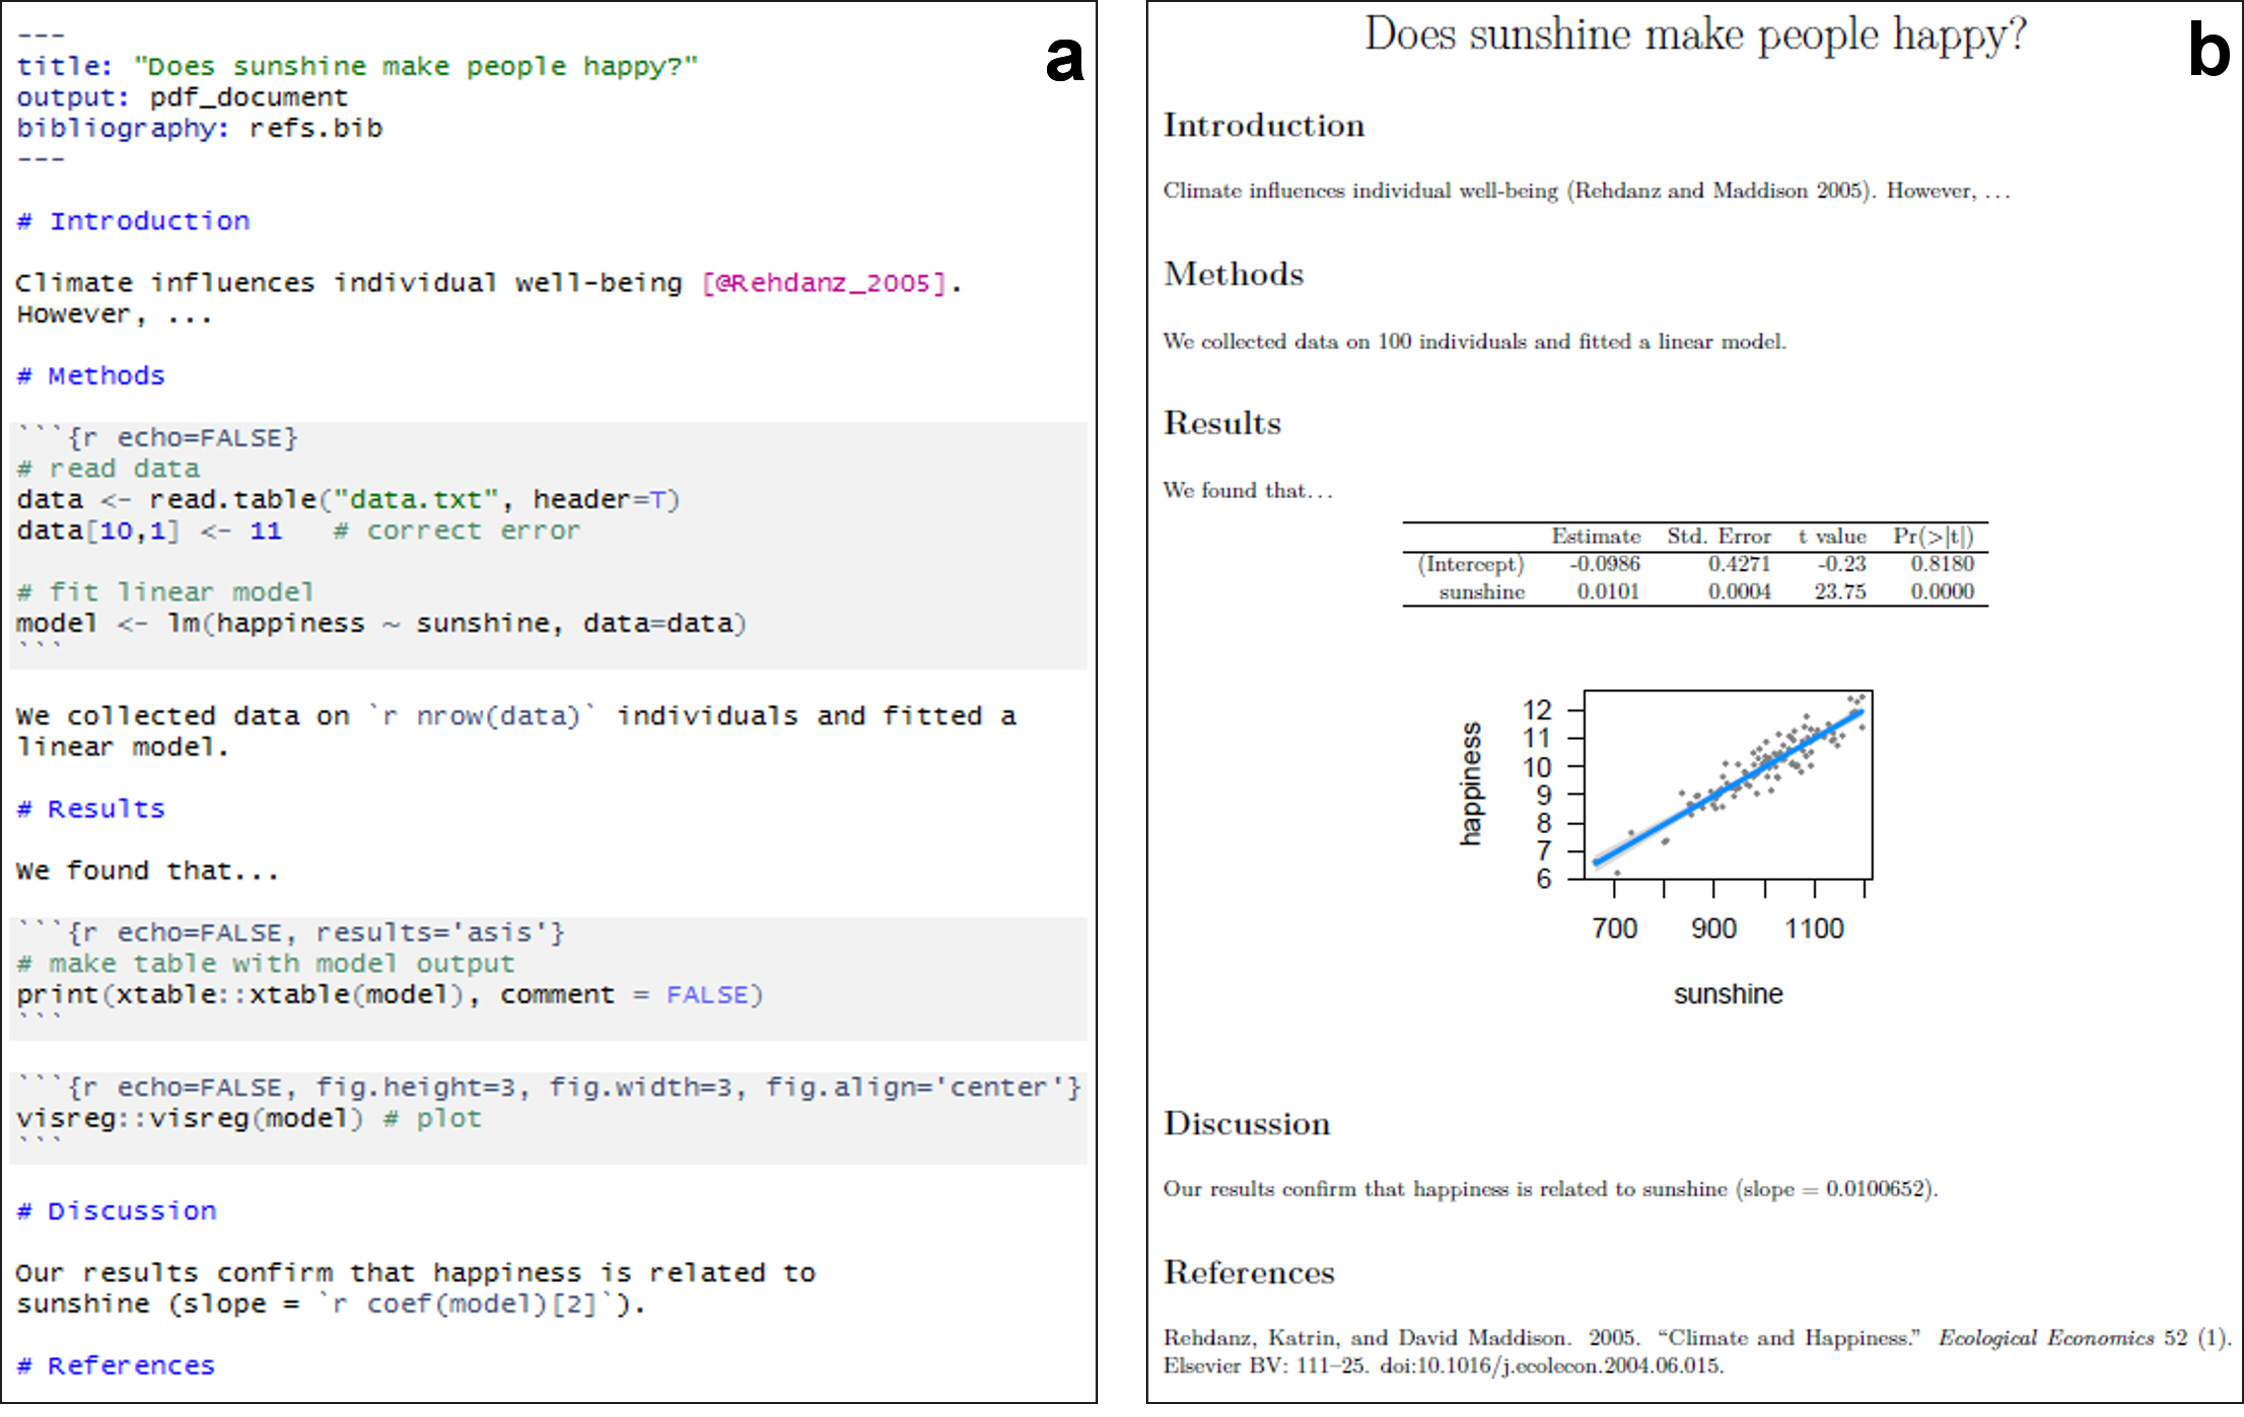
\includegraphics[width=1\linewidth]{images/fig_-002} \caption[Fig]{Fig. 3 - Ejemplo de RMarkdown.}\label{fig:unnamed-chunk-3}
\end{figure*}

En el caso concreto de R, la integración de rmarkdown en Rstudio
(www.rstudio.com) facilita la tarea de escribir artículos, tesis,
páginas web e incluso presentaciones totalmente reproducibles (véase
\url{http://rmarkdown.rstudio.com}). A modo de ejemplo, este artículo
está escrito íntegramente en Rmarkdown (véase el código fuente aquí:
\url{https://github.com/ecoinfAEET/Reproducibilidad}). Aquí
(\url{https://github.com/Pakillo/rmdTemplates}) puede descargarse una
plantilla para escribir artículos en Rmarkdown para la revista
Ecosistemas.

\hypertarget{control-de-versiones}{%
\section{Control de versiones}\label{control-de-versiones}}

``Your closest collaborator is you 6 months ago, and you don't respond
to emails.'' P. Wilson.

El control de versiones es otro de los nudos conflictivos a lo largo del
desarrollo de un proyecto. El sistema más común -y problemático- de
control de versiones consiste en guardar copias de los ficheros con
distintos nombres (Fig. 4), en un intento de tener un archivo de todos
los cambios aplicados al documento. Este sistema lleva a la acumulación
desmesurada de archivos muy similares cuyas modificaciones no son
fácilmente comparables, y dificulta reconstruir la historia del
proyecto, volver atrás en caso de detectar errores, o colaborar con
varios coautores haciendo modificaciones sobre el mismo documento.
Herramientas como Google Docs, Dropbox, Overleaf o Authorea representan
un gran avance al respecto, pero están más enfocadas a la escritura
colaborativa de manuscritos que a la integración dinámica de datos,
texto y código ejecutable como en los documentos de Rmarkdown o IPython.
Los sistemas de control de versiones se encargan de monitorizar
automáticamente los cambios realizados en cualquier fichero, registrando
quién hizo qué cambio, cuándo y por qué (Blischak et al.~2016), de forma
que es posible recuperar distintas versiones del fichero en todo
momento. En el campo de la programación exis-

Figura 3. Los documentos dinámicos que integran texto, código y
resultados (e.g.~Rmarkdown, IPython) son una herramienta revolucionaria
para hacer ciencia reproducible. Por ejemplo, un archivo Rmarkdown que
contiene texto y código (a) puede ejecutarse y producir automáticamente
documentos integrados (b) en múltiples formatos incluyendo html, pdf, o
Word. Los documentos Rmarkdown permiten trazar todo el proceso desde los
datos originales a los resultados, y son plenamente reproducibles de
manera que si hacemos cualquier cambio en los datos o el código, los
resultados se actualizan automáticamente.

Figure 3. Dynamic documents integrating text, code and results
(e.g.~Rmarkdown, IPython) are revolutionary tools for reproducible
science. For example, an Rmarkdown document (a) contaning text and code
can be automatically converted into an integrated document with text,
code and results (b) in one of multiple formats including html, pdf, and
Word. Rmarkdown documents are fully reproducible: they permit tracing
exactly how results are derived from data, and if we change anything in
the data or code, results will be updated automatically.

Figura 4. Almacenar copias de archivos con distintos nombres (a) es un
sistema de control de versiones muy ineficiente. El número de archivos
crecerá desmesuradamente, y no es fácil comparar los cambios entre
distintos archivos o reconstruir la historia del proyecto. Existen
sistemas de control de versiones muy eficientes (como git) que registran
perfectamente quién hizo qué cambio, cuándo y por qué (b). Cuando se
sincronizan con plataformas en línea como GitHub (www.github.com),
resulta muy fácil trabajar conjuntamente en proyectos incluyendo manejo
de datos, análisis y redacción de artículos.

Figure 4. Storing file copies with distinct names (a) is a very
inefficient system of version control. The number of files will grow
fast, and it is hard to compare changes between files, or navigate the
history of the project. In contrast, version control systems such as git
are very efficient to record who did what change, when, and why (b).
When used in conjunction with online platforms like GitHub
(www.github.com), it is easy to work collaborately in research projects
involving data management, analysis, and manuscript writing.

existen sistemas de control de versiones muy eficientes que
recientemente se han incorporado como herramientas básicas de la ciencia
reproducible (Ram 2013). Git (\url{https://git-scm.com/}) es el sistema
más utilizado hoy día, en conjunción con plataformas de internet como
GitHub (\url{https://github.com}), BitBucket
(\url{https://bitbucket.org/}), o GitLab (\url{https://gitlab.com/}).
Git facilita enormemente la tarea de archivar, reconstruir y navegar por
la historia de un proyecto. La integración de git en plataformas como
GitHub facilita además enormemente el desarrollo conjunto de análisis,
código y texto entre todos los colaboradores de un proyecto. A modo de
ejemplo, este artículo se escribió utilizando git para el control de
versiones y GiHub para la colaboración y discusión entre los autores. El
desarrollo completo del artículo (incluyendo quién hizo qué cambios,
cuándo y por qué) está disponible públicamente en GitHub:
\url{https://github.com/ecoinfAEET/Reproducibilidad/commits/master}.
Organización de ficheros

Mantener un sistema consistente de organizar todos los archivos
relacionados con un proyecto es otro punto importante para garantizar su
reproducibilidad (y hacer la vida del investigador más fácil). Cuando no
se tiene ningún criterio los archivos se acumulan desordenadamente y
resulta muy difícil manejar los distintos componentes del proyecto
(datos, código, figuras, texto\ldots). Esto no sólo dificulta la
comprensión y reutilización en el futuro, sino que también favorece la
aparición de errores incontrolados.

Hay muchas maneras de organizar un proyecto, y cada investigador elige
la más conveniente en su caso. Pero sí existen algunos principios
básicos (Noble 2009, véase también enlaces en Apéndice 1): (i) todos los
ficheros relacionados con el proyecto deben estar dentro del mismo
directorio (e.g.~un proyecto de Rstudio); (ii) existen subdirectorios
independientes para los datos, código, figuras, resultados y manuscrito;
(iii) los datos originales permanecen inalterados en un directorio
aparte; (iv) los datos derivados se generan mediante `scripts'; (v) las
funciones se definen en ficheros independientes del código que ejecuta
el análisis; (vi) en el directorio raíz hay un fichero README que
describe el proyecto y sus componentes, y un `script' maestro
(`makefile') que ejecuta todos los análisis.

Convenientemente, todos estos principios son compatibles con la
estructura de un paquete de R (Fig. 5). Un paquete de R no es más que
una forma estándar de organizar el código que nos permite ser más
eficientes a la hora de utilizarlo, compartirlo y editarlo (Varela
2015). Todos los paquetes de R tienen una estructura estándar con una
carpeta `R' donde residen las funciones, una carpeta `man' que contiene
los ficheros de ayuda de esas funciones, un fichero de texto `NAMESPACE'
(generado automáticamente) que especifica las funciones contenidas en el
paquete y si dependen de funciones contenidas en otros paquetes, y un
fichero `DESCRIPTION' con los metadatos del paquete: nombre, objetivos,
autores, y sus dependencias de otros paquetes. Además pueden añadirse
carpetas incluyendo archivos de datos, tests para las funciones, etc.
(Wickham 2015) por lo que la estructura, siendo estándar, mantiene su
flexibilidad.

Crear un paquete de R es mucho más fácil de lo que puede parecer (ver
Apéndice 2), y organizar un proyecto de investigación utilizando esa
estructura estándar tiene muchas ventajas (cf.~\url{https://}
github.com/ropensci/rrrpkg), entre ellas: (i) el paquete provee una
estructura de directorios para mantener los archivos organizados; (ii)
las funciones creadas para el análisis quedan documentadas, facilitando
su reutilización posterior; (iii) las funciones pueden llevar tests
asociados para comprobar que funcionan correctamente, incrementando la
robustez del análisis; (iv) se describen explícitamente las dependencias
de nuestro análisis en otros paquetes o programas externos, facilitando
la reproducibilidad del proyecto. Dependencias externas

Todo análisis reposa sobre plataformas, paquetes o programas que cambian
a lo largo del tiempo. En consecuencia, es muy frecuente que un código
deje de funcionar al introducirse cambios en alguno de los paquetes de
los que depende el proyecto (Ooms

Figura 5. Organización de directorios y archivos en un proyecto
siguiendo la estructura de un paquete de R. Los datos brutos no deben
modificarse y se encuentran separados de los datos depurados, que se
generan mediante `scripts'. Las funciones se definen en ficheros
independientes (carpeta R), y van acompañadas de documentación (carpeta
man) y tests (para comprobar que funcionan adecuadamente). Los análisis
se realizan mediante documentos Rmarkdown. Existe un script maestro
(makefile) que ejecuta el análisis (completo o por partes). Esta
estructura es flexible y puede modificarse según las preferencias del
investigador (e.g.~ver \url{https://github.com/ropensci/rrrpkg}).

Figure 5. Organisation of files and folders for a research project
following the structure of an R package. Raw data are separated from
derived (clean) data, which are obtained through scripts. Functions are
defined as independent files (R folder), have documentation (man folder)
and tests (to check that they work correctly). Analyses are done in
Rmarkdown. There is also a makefile that executes all or parts of the
analysis. This structure is flexible and highly customisable to follow
preferences of the researcher (e.g.~see
\url{https://github.com/ropensci/rrrpkg}).

2013). Igualmente, para poder reproducir un análisis en otro ordenador
habrá que instalar primero todas los programas necesarios. Por estos
motivos conviene documentar las dependencias externas de nuestro
análisis (por ejemplo qué paquetes de R se utilizan, especificando la
versión), y asegurarse de que dicho software estará disponible en el
futuro.

Hay muchas maneras posibles de registrar las dependencias de nuestro
proyecto. En R, una de las más sencillas es ejecutar la función
sessionInfo() (o su equivalente session\_info del paquete devtools) al
finalizar el análisis. Este comando devuelve un listado estructurado de
todos los paquetes utilizados, especificando su versión. Esta
información puede ser procesada directamente por paquetes como switchr
(Becker et al.~2015) para instalar todas las dependencias requeridas en
cualquier otro ordenador. Otras opciones incluyen el uso de los paquetes
rctrack (Liu y Pounds 2014), checkpoint (Revolution Analytics 2015) y
packrat (Ushey et al.~2015). Mientras rctrack y packrat almacenan una
copia local de todos los paquetes utilizados en un proyecto, checkpoint
descarga los paquetes desde un servidor de internet cuando se ejecuta.
Todos estos métodos son muy fáciles de utilizar y garantizan la
reproducibilidad de nuestro proyecto en el futuro aunque cambien los
paquetes o dependencias externas. Otras alternativas más avanzadas y
versátiles incluyen docker (Boettiger 2015) y drat (Eddelbuettel 2015).
En el Apéndice 1 hemos incluido enlaces para iniciarse en el uso de
todas ellas.

Conclusiones

La trazabilidad y reproducibilidad de los resultados científicos son
cualidades inherentes a la ciencia de calidad. Hacer ciencia de manera
reproducible no sólo es un requisito creciente en muchas revistas y
fuentes de financiación sino que además aporta muchas ventajas para el
investigador. A la larga, la ciencia reproducible ahorra tiempo y
esfuerzo, reduce el riesgo de cometer errores y aumenta el impacto y
utilidad de los trabajos en la comunidad científica.

Desarrollar estudios plenamente reproducibles requiere un esfuerzo
inicial de aprendizaje. Creemos que aquí se aplica bien la máxima de que
'es importante aprender a nadar antes de estar

hundiéndonos'. Invertir esfuerzo en adoptar flujos reproducibles puede
parecer una pérdida de tiempo al principio, pero en el futuro puede
ahorrarnos muchos problemas. El tiempo invertido en aprender a utilizar
herramientas como git o rmarkdown se ve recompensado cuando podemos
regenerar todo un manuscrito, tablas y figuras incluidas, con un solo
clic. No solo ahorramos esfuerzo, sino que nos aseguramos de que los
resultados están actualizados y libres de errores.

La transición hacia la reproducibilidad puede hacerse gradualmente. Un
buen punto de partida es la utilización de código (`scripts') para todo
el proceso de manejo y análisis de datos, así como producción de
figuras. Este código debe ser capaz de generar los resultados finales a
partir de los datos originales, y ambos pueden publicarse junto con el
manuscrito para hacerlo más reproducible. Igualmente, podríamos empezar
a utilizar repositorios de datos en la nube (e.g.~Open Science
Framework, Figshare) para almacenar, versionar y compartir nuestros
datos. El siguiente paso podría ser estructurar nuestro código en un
documento dinámico (Rmarkdown/IPython). Finalmente puede incorporarse un
sistema de control de versiones (e.g.~git/GitHub) para guardar un
registro del desarrollo del proyecto y facilitar la colaboración con
otros investigadores.

Esperamos que este artículo anime a muchos investigadores a adoptar
estas prácticas, y que las pautas y recursos aquí recogidos faciliten la
transición hacia una ciencia más reproducible.

Agradecimientos

FRS está financiado por una ayuda de formación postdoctoral del
Ministerio de Economía y Competitividad. SV tiene un contrato
postdoctoral del programa propio de la Universidad de Alcalá. Los
autores desean agradecer expresamente a todos los programadores,
instituciones y empresas que hacen posible, muchas veces de manera
altruista, la ciencia reproducible.

Referencias

Alberts, B., Cicerone, R.J., Fienberg, S.E., Kamb, A., McNutt, M.,
Nerem, R.M., Schekman, R. et al.~2015. Self-correction in science at
work. Science 348: 1420-1422. Alonso, B., Valladares, F. 2006. Bases de
datos y metadatos en ecología: compartir para investigar en cambio
global. Ecosistemas 15: 1-6. Anónimo 2014a. Code share. Nature 514:
536-536.

Anónimo 2014b. Journals unite for reproducibility. Nature 515: 7-7.

Bass, B., Nixon, T. 2008. Computer languages. En Jorgensen, S., Fath, B.
(eds.), Encyclopedia of ecology, pp.~720-731. Becker, G., Barr, C.,
Gentleman, R., Lawrence, M. 2015. Enhancing reproducibility and
collaboration via management of R package cohorts. Arxiv,
\url{http://arxiv.org/abs/1501.02284v2}.

Blischak, J.D., Davenport, E.R., Wilson, G. 2016. A Quick Introduction
to Version Control with Git and GitHub. PLOS Computational Biology 12:
e1004668. Boettiger, C. 2015. An introduction to Docker for reproducible
research. ACM SIGOPS Operating Systems Review 49: 71-79.

Bond-Lamberty, B. 2014. Robust and reproducible research using R.
\url{http://rstudio-pubs-static.s3.amazonaws.com/14911_24ffedb}
113f74789b709cbd694dc255c.html\#/

Check Hayden, E. 2015. Rule rewrite aims to clean up scientific
software. Nature 520: 276-277.

Claerbout, J., Karrenbach, M. 1992. Electronic documents give
reproducible research a new meaning. En: Proceedings of the 62nd annual
international meeting of the society of exploration geophysics, Octubre
1992, New Orleans, Estados Unidos. pp.~601-604.

Eddelbuettel D. 2015. drat: Drat R Archive Template.
\url{https://cran.rproject.org/package=drat}.

Fegraus, E.H., Andelman, S., Jones, M.B., Schildhauer, M. 2005.
Maximizing the Value of Ecological Data with Structured Metadata: An
Introduction to Ecological Metadata Language (EML) and Principles for
Metadata Creation. The Bulletin of the Ecological Society of America 86:
158-168.

Rodríguez-Sánchez et al.~2016 FitzJohn, R.G., Pennell, M.W., Zanne,
A.E., Stevens, P.F., Tank, D.C., Cornwell, W.K. 2014. How much of the
world is woody? Journal of Ecology 102: 1266-1272.

Garijo, D., Kinnings, S., Xie, L., Xie, L., Zhang, Y., Bourne, P.E.,
Gil, Y. 2013. Quantifying Reproducibility in Computational Biology: The
Case of the Tuberculosis Drugome. PLoS ONE 8: e80278.

Goring, S., Lacourse, T., Pellatt, M.G., Mathewes, R.W. 2013. Pollen
assemblage richness does not reflect regional plant species richness: a
cautionary tale. Journal of Ecology 101: 1137-1145.

Hampton, S.E., Anderson, S.S., Bagby, S.C., Gries, C., Han, X., Hart,
E.M., Jones, M.B. et al.~2015. The Tao of open science for ecology.
Ecosphere 6: art120. Hart, E., Barmby, P., LeBauer, D., Michonneau, F.,
Mount, S., Mulrooney, P., Poisot, T. et al.~2016. Ten simple rules for
digital data storage. Peer J preprints 4: e1448v2.

Ince, D.C., Hatton, L., Graham-Cumming, J. 2012. The case for open
computer programs. Nature 482: 485-488.

Liu, Z., Pounds, S. 2014. An R package that automatically collects and
archives details for reproducible computing. BMC Bioinformatics 15: 138.
Markowetz, F. 2015. Five selfish reasons to work reproducibly. Genome
Biology 16: 274.

Marwick, B. 2016. Computational Reproducibility in Archaeological
Research: Basic Principles and a Case Study of Their Implementation.
Journal of Archaeological Method and Theory 23(2): 1--27.

Michener, W.K. 2015. Ten Simple Rules for Creating a Good Data
Management Plan. PLoS Computational Biology 11: 1-9.

Michener, W.K., Brunt, J.W., Helly, J.J., Kirchner, T.B., Stafford, S.G.
1997. Nongeospatial metadata for the ecological sciences. Ecological
Applications 7: 330-342. Michener, W.K., Jones, M.B. 2012.
Ecoinformatics: supporting ecology as a data-intensive science. Trends
in Ecology and Evolution 27: 85-93.

Noble, W.S. 2009. A Quick Guide to Organizing Computational Biology
Projects. PLoS Computational Biology 5: e1000424. Ooms, J. 2013.
Possible Directions for Improving Dependency Versioning in R. The R
journal 5: 197-206.

Peng, R.D. 2011. Reproducible Research in Computational Science. Science
334: 1226-1227.

Pigliucci, M., Boudry, M. 2013. Philosophy of pseudoscience:
reconsidering the demarcation problem. University of Chicago Press,
Chicago, IL, Estados Unidos.

Piwowar, H.A., Day, R.S., Fridsma, D.B. 2007. Sharing Detailed Research
Data Is Associated with Increased Citation Rate. PLoS ONE 2: e308.

Ram, K. 2013. Git can facilitate greater reproducibility and increased
transparency in science. Source Code for Biology and Medicine 8: 7.
Revolution Analytics 2015. checkpoint: Install Packages from Snapshots
on the Checkpoint Server for Reproducibility.
\url{https://cran.r-project.org/} package=checkpoint.

Rüegg, J., Gries, C., Bond-Lamberty, B., Bowen, G.J., Felzer, B.S.,
McIntyre, N.E., Soranno, P.A. et al.~2014. Completing the data life
cycle: using information management in macrosystems ecology research.
Frontiers in Ecology and the Environment 12: 24-30. Stodden, V., Guo,
P., Ma, Z. 2013. Toward Reproducible Computational Research: An
Empirical Analysis of Data and Code Policy Adoption by Journals. PLoS
ONE 8: e67111.

Ushey, K., McPherson, J., Cheng, J., Atkins, A., Allaire, J.J. 2015.
packrat: A Dependency Management System for Projects and their R Package
Dependencies. \url{https://cran.r-project.org/package=packrat}.

Vanderbilt, K.L., Lin, C.-C., Lu, S.-S., Kassim, A.R., He, H., Guo, X.,
Gil, I.S. et al.~2015. Fostering ecological data sharing: collaborations
in the International Long Term Ecological Research Network. Ecosphere 6:
1-18.

Vandewalle, P. 2012. Code Sharing Is Associated with Research Impact in
Image Processing. Computing in Science and Engineering 14: 42-47.

Varela, S. 2015. «R packages. Organize, test, document, and share your
code», de Hadley Wickham. Ecosistemas 24: 103.

Vines, T.H., Albert, A.Y., Andrew, R.L., Débarre, F., Bock, D.G.,
Franklin, M.T., Gilbert, K.J. et al.~2014. The Availability of Research
Data Declines Rapidly with Article Age. Current Biology 24: 94-97.

White, E., Baldridge, E., Brym, Z., Locey, K., McGlinn, D., Supp, S.
2013. Nine simple ways to make it easier to (re)use your data. Ideas in
Ecology and Evolution 6: 1-10.

Wickham, H. 2015. R packages: organize, test, document, and share your
code. O'Reilly Media, In., Sebastopol, CA. Estados Unidos. Wickham, H.
2014. Tidy Data. Journal of Statistical Software 59: 1-23.

Apéndice 1. Recursos sobre ciencia reproducible. Appendix 1. Resources
for reproducible science. Recursos generales sobre reproducibilidad

Control de versiones (Git \& GitHub)

Reproducible research in computational science

•

Ten simple rules for reproducible computational research

•

Nature special: Challenges in irreproducible research Best practices for
scientific computing

Good enough practices for scientific computing Initial steps toward
reproducible research Tools for reproducible research

The tao of open science for ecology

Towards standard practices for sharing computer code and programs in
neuroscience Reproducible research is still a challenge rOpenSci
reproducibility guide

Reproducible research course

Report writing for data science in R

Implementing reproducible research

Reproducible Research with R and Rstudio Digital History Methods in R

Doing reproducible science: from your hard-won data to a publishable
manuscript without going mad

Manejo de datos •

A guide to data management in ecology and evolution (British Ecological
Society)

•

Ten simple rules for the care and feeding of scientific data

•

Ecoinformatics: supporting ecology as a data-intensive science Ten
simple rules for digital data storage

Nine simple ways to make it easier to (re)use your data

Ten simple rules for creating a good data management plan Data
Management Planning Tool

Ejemplo de data management plan Bad data guide

Data Carpentry Spreadsheets for Ecology DataONE Best Practices Tidy data

Spreadsheet help Data organization

Repositorios de datos

Open Science Framework

Paquetes de rOpenSci para publicación de datos

Paquete de R para interaccionar con Open Science Framework Ecological
Metadata Language

Análisis de datos y documentos dinámicos •

knitr

•

IPython

•

Jupyter

•

Dynamic documents with R and knitr

•

A Quick Introduction to Version Control with Git and GitHub

•

Git and GitHub (Hadley Wickham)

•

Git can facilitate greater reproducibility and increased transparency in
science Working with RStudio, Git, GitHub (STAT 545) Version control
with git (R. Fitzjohn)

Version control with Git (Software Carpentry)

A basic tutorial to version control using git (Jon Lefcheck) Push, Pull,
Fork - GitHub for academics

Git for beginners - the definitive practical guide (Stackoverflow) Git -
the simple guide

Code School Git intro

GitHub tutorial (Karl Broman) Getting git right (Atlassian)

Hello World (GitHub first steps) GitHub guides

Organización de proyectos y creación de paquetes •

A quick guide to organizing computational biology projects

•

Designing projects

•

Reproducible Research Project Initialization Rstudio projects

Using R packages as research compendiums R packages (H. Wickham) R
packages (K. Broman) Choose a license

A minimal tutorial on make (K. Broman) remake

Manejo de dependencias •

rctrack: An R package that automatically collects and archives details
for reproducible computing

•

packrat: reproducible package management for R

•

•

•

•

•

checkpoint package

Enhancing reproducibility and collaboration via management of R package
cohorts An introduction to Docker for reproducible research R Docker
tutorial

drat: R repositories made easy

Para un listado actualizado, consultar
\url{https://github.com/ecoinfAEET/Reproducibilidad}

rmarkdown

•

Interactive notebooks: sharing the code Report writing for data science
in R

Implementing reproducible research

Reproducible Research with R and Rstudio

Apéndice 2. Creación de Paquetes R Appendix 2. Creating R packages

Estructura estándar de un paquete de R

De manera general un paquete de R es una carpeta que debe tener al menos
3 subcarpetas (R, man y tests/testthat) y dos archivos de texto
(DESCRIPTION y NAMESPACE). R

En esta carpeta se guardan los archivos .R definiendo las funciones.
Cada función deberá llevar escrita su documentación inmediatamente
encima de ella usando roxygen2 (ver ejemplo). Además tendremos que crear
un archivo .R llamado myfirstpackage-package.R en donde expliquemos, de
nuevo usando roxygen2, qué hace y cómo funciona nuestro paquete
(ejemplo).

man

En esta carpeta se guardarán los archivos .Rd, es decir, los archivos de
ayuda que explican todos los detalles de la función. Estos archivos se
abren cuando se usa la función ? y además forman el manual oficial del
paquete en pdf. Estos archivos no se deben escribir a mano sino que se
crean automáticamente cuando se ejecuta el comando roxygenize (ejemplo).

tests/testthat

Además, debemos incorporar tests para cada función para comprobar que
están funcionando bien y haciendo lo que realmente queremos. Los test
son scripts de R que comprueban cada función (son archivos .R, ver
\url{https://cran.r-project.org/web/packages/testthat/testthat.pdf}).
Estos tests son fundamentales a la hora de mantener un paquete porque
cuando los paquetes crecen y se hacen complejos las interdependencias
entre funciones son menos evidentes, así que podríamos llegar a
modificar una función sin darnos cuenta de que al hacerlo estamos
rompiendo otra que depende de ella (y las razones pueden no ser
evidentes a primera vista, e.g., cuestiones de formato de los datos)
(ejemplo). DESCRIPTION

Es un archivo de texto en el cual se especifica el nombre del paquete,
su versión, los autores, emails, las dependencias que tiene, etc.
(ejemplo).

NAMESPACE

Es un archivo de texto que se genera automáticamente al ejecutar el
comando roxygenize en el cual se especifican los nombres de las
funciones que estarán disponibles al cargar nuestro paquete, incluyendo
funciones propias del paquete y funciones importadas de otros paquetes.
Si nuestro paquete tiene una función con el mismo nombre que otro que se
haya cargado antes, R genera un mensaje informando del problema
(colisión de nombres). Para evitar colisiones de nombres se puede
aplicar un prefijo de forma que los nombres de las funciones no
coincidan con los de ninguna otra función que haya sido programada en R.

Crear el paquete

Finalmente, después de haber ejecutado el comando roxygenize para
generar los manuales y el NAMESPACE, podemos crear nuestro paquete
ejecutando: R CMD build --resave-data myfirstpackage

Si nuestro paquete pasa el check --as-cran sin ningún problema podríamos
incluso compartirlo en el repositorio CRAN de R. R CMD check --as-cran
myfirstpackage\_0.1.tar.gz

Evidentemente hay muchos más elementos que pueden añadirse a un paquete.
Aquí hay una guía muy completa y sencilla para crear paquetes.

This document is also available in
\href{https://rstudio.github.io/tufte/cn/}{Chinese}, and its
\texttt{envisioned} style can be found
\href{https://rstudio.github.io/tufte/envisioned/}{here}.

\bibliography{skeleton.bib}



\end{document}
